\documentclass{article}
\usepackage[utf8]{inputenc}
\usepackage[T1]{fontenc}
\usepackage[english]{babel} % Changed to English
\usepackage{microtype}
\usepackage{graphicx}
\usepackage{float}
\usepackage{subcaption}
\usepackage{hyphenat}
\usepackage{natbib}
\usepackage{url}
\usepackage{amsmath}
\usepackage{booktabs}
\usepackage{caption} % Added for caption spacing control
\captionsetup{skip=5pt} % Reduces space between figure content and caption

\begin{document}

\title{AI-Based IGRT with 2D Image-Guided Dose Tracking of Daily Cone-Beam CTs
for Assessing Prostate Position, Rectum, and Bladder Filling in Definitive
Radiotherapy of Prostate Carcinoma}
\author{\begin{minipage}{0.8\textwidth}\centering\small Peter Rhone,
Dipl.-Phys., Prof. Dr. med. Thomas Kuhnt, \\ Dr. med. Franziska
Nägler\end{minipage}}
\maketitle

\vspace{2cm}

\begin{abstract}
A method for the automatic detection of the bladder and rectum in daily
Cone-Beam CTs (kV-CBCTs) for image-guided radiotherapy (IGRT) is presented.
Medial sagittal slices – centered through the symphysis and one each to the left
and right – were segmented using artificial intelligence (AI) to evaluate organ
position and the filling states of the rectum and bladder during definitive
radiotherapy of prostate carcinoma. The model was trained and validated with
data from 131 patients (5 CBCTs per patient). The results demonstrate high
segmentation accuracy with Dice coefficients of approximately 0.98 for the
bladder and prostate PTV, and 0.95 for the rectum.  \end{abstract}

\section{Introduction}
In the definitive irradiation of low- and intermediate-risk prostate carcinomas,
curative doses of 68~Gy are applied in moderate hypofractionation at our
institution \citep{ethik2024}. Intrafractional variability, such as filling
states or organ motion, can lead to risk organs like the bladder and rectum
receiving undesirably high doses, potentially increasing acute or chronic
toxicity \citep{kupelian2007, quantec}. Image-guided radiotherapy (IGRT) with
Cone-Beam CTs (CBCTs) verifies organ positions before each fraction. However,
varying filling states – such as a poorly filled bladder or an air-filled rectum
– complicate adherence to dose constraints like \( V_{65} < 50\,\% \) for the
bladder \citep{wang2022, quantec}. Online adaptive radiotherapy enables daily
adaptation to these changes but requires significant personnel effort (15–35
minutes per fraction) \citep{byrne2022}, which is hardly feasible in
high-throughput clinics. Often, only an offline review is performed, identifying
deviations only after the fact. This study develops an AI-based method for
partially automating online adaptive therapy, inspired by advances in medical
image segmentation \citep{litjens2017}, to more efficiently monitor prostate
position and organ filling and improve treatment quality.

\section{Methods}
Between July 1, 2019, and January 31, 2024, 131 patients with low- to
intermediate-risk prostate carcinoma who received definitive, moderately
hypofractionated radiotherapy (25 fractions, 58–68\,Gy) were retrospectively
selected \citep{ethik2024}. Inclusion criteria included cT1a–cT2b, PSA \(\leq
20\,\text{ng/ml}\), and Gleason Score \(\leq 7\); patients with high-risk
profiles or distant metastases were excluded. Written consent for anonymized
data use was obtained.

For each patient, a planning CT (PL-CT) and 5 kV-CBCTs were anonymously
extracted from the RayStation system (versions 10B–12A) \citep{zwart2022}.
Structures (prostate PTV, bladder, rectum, etc.) were manually contoured by a
medical physicist and reviewed by a specialist physician. A Python program
(\textit{sqlite\_dicom2.py}) converted DICOM data into volumes, extracted three
medial sagittal 2D slices per CBCT – a central slice through the symphysis and
one each to the left and right – and generated binary masks of the contours
using \textit{scipy.ndimage.ConvexHull}. The outputs (patient number, DICOM
series, slice images, mask, slice number) were stored in an SQLite database. A
second program (\textit{sqlite\_viewer.py}) facilitated visual inspection and
data cleaning.

The images were preprocessed (removal of unusually sized images, normalization
of pixel data). In total, approximately 2100 images per organ were generated (3
slices × 5 CBCTs × 131 patients), of which about 1700 were used for training and
400 for validation. Patients whose images were used for training were excluded
from the validation dataset. To enhance quality, the 1700 training images were
augmented – random rotation, scaling, translation, and noise – resulting in
approximately 9000 images, a proven method for improving model robustness in
image segmentation \citep{ronneberger2015, pereira2016, shorten2019}.

A Convolutional Neural Network (CNN) based on U-Net \citep{ronneberger2015} was
trained using PyTorch, accelerated by the ROCm stack on an AMD RX 7900 XTX GPU
with 24 GB VRAM. The model consists of an encoder-decoder architecture with
convolutional blocks (each with two \(3 \times 3\) convolutions with ReLU
activation) and transposed convolutions for upsampling layers. It was trained
with a learning rate of \(10^{-4}\) and the Adam optimizer over 25 epochs, using
binary cross-entropy with logits (\textit{BCEWithLogitsLoss}) as the loss
function. Only CBCT data were used for training to ensure consistency
\citep{litjens2017}. Training data were organized in a custom
\textit{ImageDataset} as PyTorch tensors (stacked from Pandas Series) and loaded
with a \textit{DataLoader} (batch size 32, 4 workers,
\textit{pin\_memory=True}). During training, images and masks were moved to the
GPU in batches, with the loss backpropagated and optimized after each batch.
Training time was approximately 1 hour per organ.

Bladder volume was roughly estimated by measuring the height and width of the
bladder mask in the central sagittal plane and calculating the volume of a
prolate spheroid. For the rectum, the volume of a cylinder was used for
estimation.

\section{Results}
The U-Net model was tested on approximately 400 validation images per organ. The
segmentation accuracy yielded the following Dice coefficients, averaged over all
validation images:

\begin{table}[H]
  \centering
  \begin{tabular}{lc}
    \toprule
    Organ & Dice Coefficient \\
    \midrule
    Bladder         & $0.9815 \pm 0.0126$ \\
    Prostate PTV    & $0.9789 \pm 0.0092$ \\
    Rectum          & $0.9552 \pm 0.1021$ \\
    \bottomrule
  \end{tabular}
  \caption{Dice coefficients with standard deviations for various organs.}
  \label{tab:dice_coefficients}
\end{table}

The volumes of the bladder and rectum were estimated. These values can be
compared with the volumes from the PL-CT to assess filling states.

Manually created contours, reviewed by a specialist physician, served as the
"Ground Truth." Model predictions were visually compared with the Ground Truth
data. Examples are shown in Figures \ref{fig:bladder_combined},
\ref{fig:prostate_combined}, and \ref{fig:rectum_combined}.

\begin{figure}[H]
    \centering
    \begin{subfigure}[t]{0.9\textwidth}
        \centering
        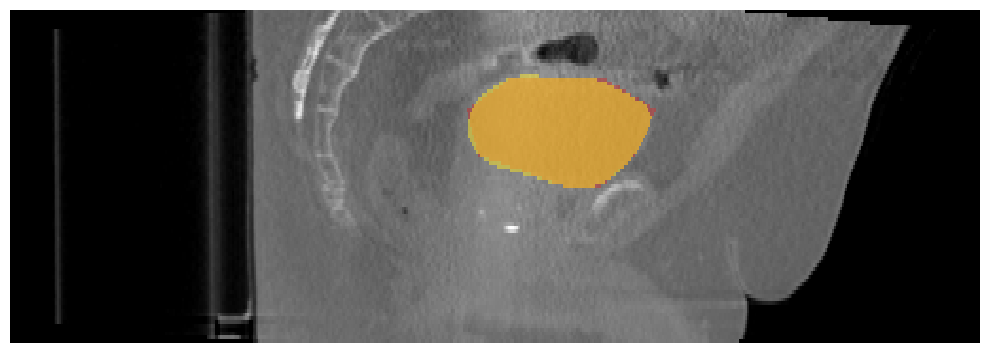
\includegraphics[width=\textwidth]{images/bladder_merged.png}
        \caption{Example segmentation of the bladder. Orange: Ground Truth,
        Yellow: Prediction.} \label{fig:harnblasen_segmentation_merged}
    \end{subfigure}
    \begin{subfigure}[t]{0.9\textwidth}
        \centering
        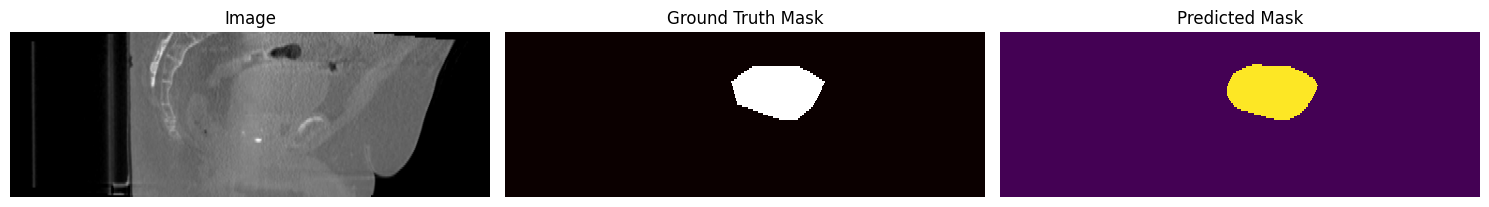
\includegraphics[width=\textwidth]{images/bladder_3_panel.png}
        \caption{Example segmentation of the bladder. Left: Original image,
        Center: Ground Truth, Right: Model prediction.}
        \label{fig:harnblasen_segmentation}
    \end{subfigure}
    \caption{Overview of segmentation results for the bladder.}
    \label{fig:bladder_combined}
\end{figure}

In Figure \ref{fig:harnblasen_segmentation}, the segmentation visibly covers the
bladder better than the Ground Truth, which appears jagged due to segmentation
artifacts. The model prediction is smoother and fully encompasses the bladder.
The bladder filling in this example was estimated at 150\,ml.

\begin{figure}[H]
    \centering
    \begin{subfigure}[t]{0.9\textwidth}
        \centering
        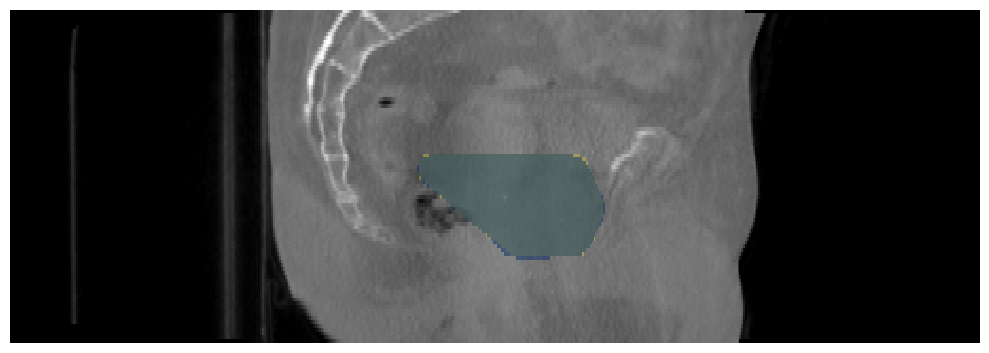
\includegraphics[width=\textwidth]{images/prostate_merged.png}
        \caption{Example segmentation of the prostate PTV. Yellow: Ground Truth,
        Blue: Prediction.} \label{fig:prostata_segmentation_merged}
    \end{subfigure}
    \begin{subfigure}[t]{0.9\textwidth}
        \centering
        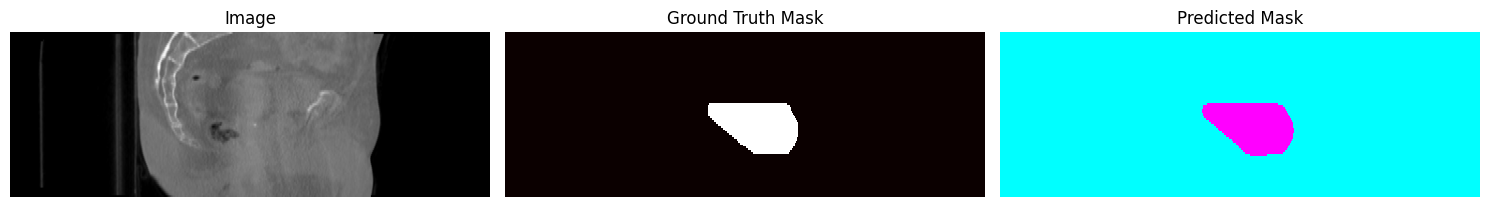
\includegraphics[width=\textwidth]{images/prostate_3_panel.png}
        \caption{Example segmentation of the prostate PTV. Left: Original image,
        Center: Ground Truth, Right: Model prediction.}
        \label{fig:prostata_segmentation}
    \end{subfigure}
    \caption{Overview of segmentation results for the prostate PTV.}
    \label{fig:prostate_combined}
\end{figure}

The model prediction in Figure \ref{fig:prostata_segmentation} covers the
prostate PTV very well. This is of optional interest, as the PTV lacks clearly
defined anatomical boundaries like the bladder. Nevertheless, the actual PTV can
be overlaid on the CBCT to estimate the dose delivered to risk organs.

\begin{figure}[H]
    \centering
    \begin{subfigure}[t]{0.9\textwidth}
        \centering
        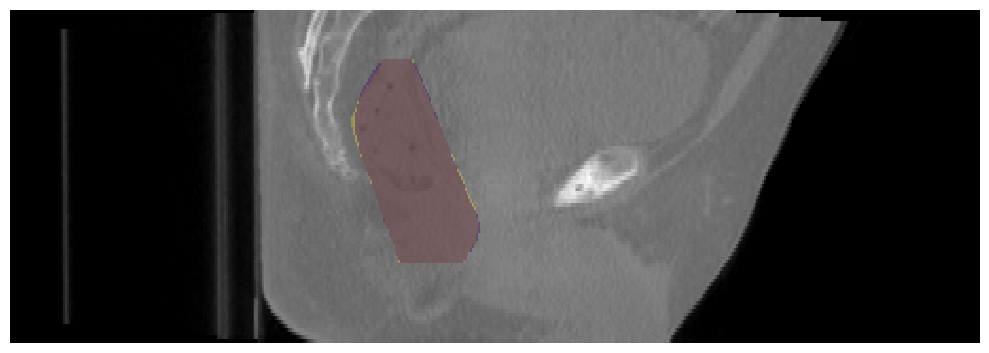
\includegraphics[width=\textwidth]{images/rectum_merged.png}
        \caption{Example segmentation of the rectum. Yellow: Ground Truth,
        Brown: Prediction.} \label{fig:rektum_segmentation_merged}
    \end{subfigure}
    \begin{subfigure}[t]{0.9\textwidth}
        \centering
        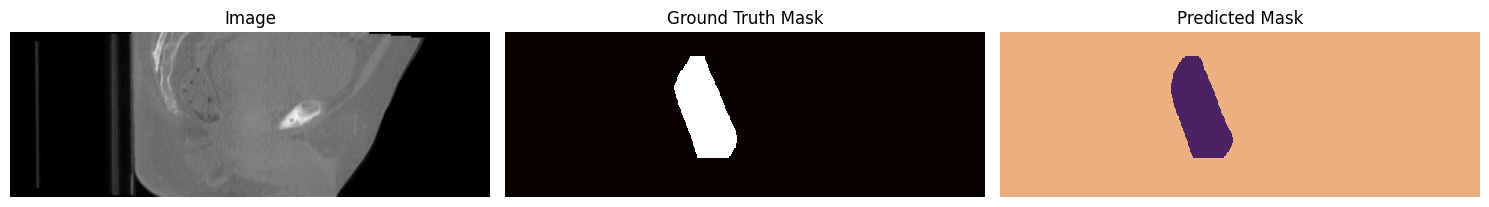
\includegraphics[width=\textwidth]{images/rectum_3_panel.png}
        \caption{Example segmentation of the rectum. Left: Original image,
        Center: Ground Truth, Right: Model prediction.}
        \label{fig:rektum_segmentation}
    \end{subfigure}
    \caption{Overview of segmentation results for the rectum.}
    \label{fig:rectum_combined}
\end{figure}

The results for the rectum in Figure \ref{fig:rektum_segmentation} are also
satisfactory, though less precise than for the bladder and prostate PTV. This is
reflected in the lower Dice coefficient and higher standard deviation. The
rectum filling in this example was estimated at 300\,ml.

\section{Discussion}
The method enables precise segmentation of the bladder and rectum. The Dice
coefficient of approximately 0.98 for the bladder and prostate PTV provides
reliable results for daily use. The value of approximately 0.95 for the rectum
is also acceptable, particularly in conjunction with visualization. The higher
standard deviation of approximately 0.1 for the rectum reflects its greater
variability \citep{litjens2017}. The trained models can be executed on a
standard computer in a few seconds (near real-time), enabling integration into
clinical workflows, such as a plugin for the RayStation system.

Extending the model to the full kV-CBCT volume would allow 3D segmentation of
risk organs, enhancing the method’s accuracy and robustness. Direct measurement
of organ volumes would be particularly useful. However, this would likely
require a larger dataset and more computational power.

Limitations of the method include dependence on consistent CBCT parameters and
the inaccuracy due to information loss from dimensionality reduction to 2D.

Future work could employ transfer learning or advanced augmentation to improve
robustness against variable devices.

\section{Conclusion}
The AI-based method effectively automates the verification of prostate position
and organ filling, offering potential to enhance treatment quality and
efficiency in IGRT. The high Dice coefficients support the possibility of use
without fiducials (e.g., gold markers) in the prostate, as is currently common.
It lays the foundation for broader clinical applications following further
validation.

\section{Acknowledgments}
We thank the Department of Radiation Therapy at the University Hospital Leipzig
for providing data and technical support, as well as Prof. Dr. med. Thomas Kuhnt
and Dr. med. Franziska Nägler for professional guidance, and Saskia Spautz for
preparing the patient data.

\section{References}
\bibliographystyle{plainnat}
\bibliography{references}

\end{document}